\section{The Path Integral}

\begin{definition}
    We define a \textbf{path} on $\C$ to be a continuous complex valued
    functiom $\y:[a,b] \xrightarrow{} \C$. We call $\y(a)$ the \textbf{initial
    point} of $\y$ and $\y(b)$ the \textbf{end point} of $\y$. We define the
    \textbf{trace} of $\y$ to be the image of  $\y$  (i.e. $\y([a,b])$) and
    denote it $\{\y\}$. We call the path $\y$  \textbf{closed} if $\y(a)=\y(b)$.
\end{definition}

\begin{definition}
    We call a path $\y:[a,b] \xrightarrow{} \C$ \textbf{rectifiable} if it is of
    bounded variation. Moreover, if $\y$ is piecewise $C^1$, we  define the
    \textbf{length} of $\y$ to be the total variation of $\y$; that is
    \begin{equation*}
        l(t)=\int_a^b{|\y'(t)| \ dt}
    \end{equation*}
\end{definition}

\begin{figure}[h]
    C\centering
    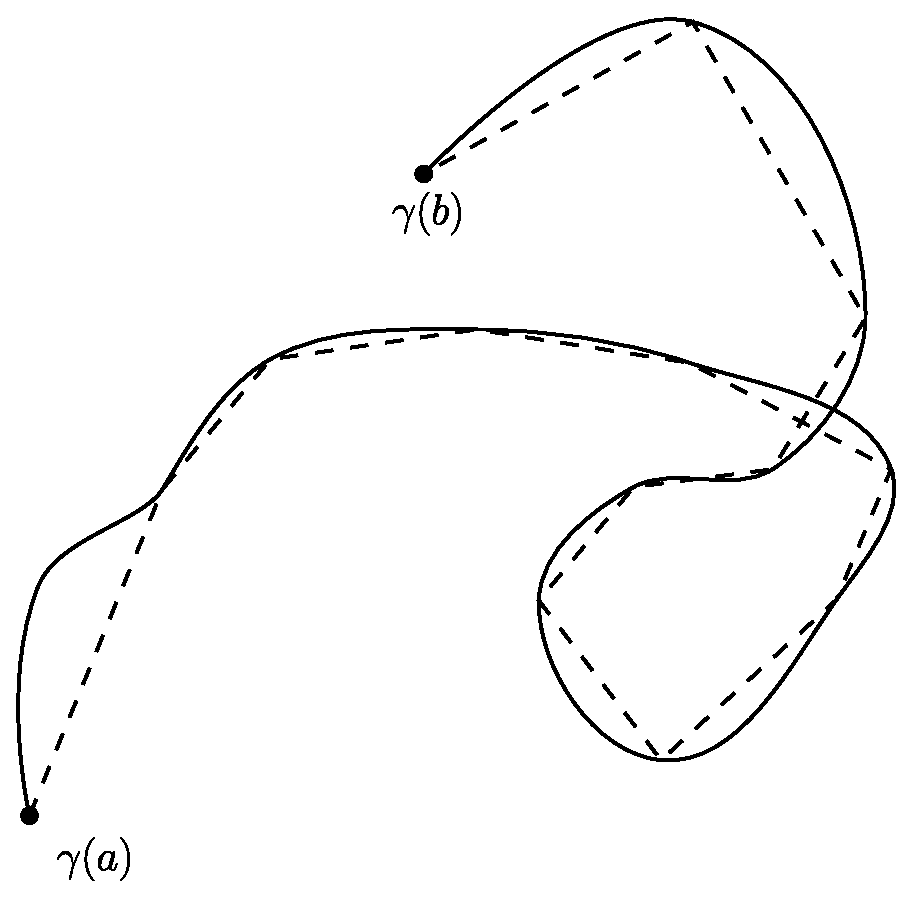
\includegraphics[scale=0.5]{Figures/Chapter4/rectifiable_curve.eps}
    \caption{A rectifiable path in $\C$.}
    \label{figure_4.1}
\end{figure}

\begin{definition}
    If $\y:[a,b] \xrightarrow{} \C$ is a rectifiable path in $\C$, and $f$ is a
    continuous complex valued function defined on  $\{\y\}$, then the
    \textbf{path integral} of $f$  \textbf{along} $\y$ is defined to be
    \begin{equation*}
        \int_\y{f(z) \ dz}=\int_a^b{f \circ \y(t) \ d\y}
    \end{equation*}
\end{definition}

\begin{example}\label{example_4.1}
    \begin{enumerate}
        \item[(1)] Take $\y:[0,2\pi] \xrightarrow{} \C$ by $\y(t)=e^{it}$ and
            consider $f(z)=\frac{1}{z}$ defined on $\com{\C}{\{0\}}$. Then $\y$
            is differentiable, and a rectifiable path, so that
            \begin{equation*}
                \int_\y{\frac{dz}{z}}=i\int_0^{2\pi}{dt}=2i\pi
            \end{equation*}

        \item[(2)] Let $m \geq 0$, and  $\y(t)=e^{it}$ on $0 \leq t \leq 2\pi$.
            Then
            \begin{equation*}
                \int_\y{z^m \ dz}=i\int_0^{2\pi}{e^{imt}e^{it}}=0
            \end{equation*}

        \item[(3)] Let $n \geq 0$ and $\y(t)=tb+(1-t)a$ on $0 \leq t \leq 1$,
            for $a,b \in \C$. Then
            \begin{equation*}
                \int_\y{z^n \ dz}=(b-a)\int_0^1{(tb-(1-t)a)^t \ dt}=
                \frac{b^{n+1-a^{n+1}}}{n+1}
            \end{equation*}
    \end{enumerate}
\end{example}

\begin{lemma}\label{4.2.1}
    If $\y:[a,b] \xrightarrow{} \C$ is a recitifiable path and $\phi:[c,d]
    \xrightarrow{} [a,b]$ is a nondecreasing function who's image is $[a,b]$,
    then $\y \circ \phi:[c,d] \xrightarrow{} \C$ is a rectifiable path with
    trace $\{\y \circ \phi\}=\{\y\}$.
\end{lemma}

\begin{theorem}\label{4.2.2}
    If $\y:[a,b] \xrightarrow{} \C$ is a rectifiable path, and $\phi:[c,d]
    \xrightarrow{} [a,b]$ is a nondecreasing function who's image is $[a,b]$,
    the for every continuous complex valued function $f$ defined on  $\{\y\}$,
    \begin{equation*}
        \int_\y{f}=\int_{\y \circ \phi}{f}
    \end{equation*}
\end{theorem}
\begin{proof}
    Let $\e>0$ and choose a  $\d_1>0$ and $S=\{c=s_0<\dots<s_n=d\}$ a
    partition of $[c,d]$ such that $\|S\|<\d_1$ and $s_k \leq \s_k \leq
    \s_{k+1}$. We then get
    \begin{equation*}
        \Big{|} \int_{\y \circ \phi}{f}-
        \sum_{k=0}^{n-1}{f(\y \circ \phi(\s_k))
            (\y \circ \phi(s_{k+1})-\y \circ \phi(s_k))} \Big{|}<\frac{\e}{2}
    \end{equation*}
    Choose $\d_2>0$ and $T=\{a=t_0<\dots<t_m=b\}$ a partion of $[a,b]$ such that
    $\|T\|<\d_2$ and $t_k \leq \t_l \leq t_{l+1}$. Then
    \begin{equation*}
        \Big{|} \int_\y{f}-\sum_{l=0}^{m-1}{f(\t_l)(\y(t_{l+1})-\y(t_l))} \Big{|}
        < \frac{\e}{2}
    \end{equation*}
    Since $\phi$ is continuous on $[c,d]$, it is uniformly continuous, so that
    there exists a $\d>0$ chosen such that $\d=\min{\{\d_1,\d_2\}}$ and for
    which $|\phi(s)-\phi(s')|<\e$ whenever $0<|s-s'|<\d$. Then if $\|S\|<\d$,
    and  $t_l=\phi(s_k)$, then $\|T\|<\d$ and if $s_k \leq \s_k \leq s_{k+1}$
    with $\t_l=\phi(\s_k)$, then we get
    \begin{equation*}
        \Big{|} \int_\y{f}-\int_{\y \circ \phi}{f} \Big{|}<\e
    \end{equation*}
\end{proof}

\begin{definition}
    Let $\s:[a,b] \xrightarrow{} \C$ and $\y:[a,b] \xrightarrow{} \C$ be
    rectifiable paths. If $\phi:[a,b] \xrightarrow{} [a,b]$ is a continuous
    strictly increasing functuion who's image is $[a,b]$, such that $\s=\y \circ
    \phi$, then we call  $\phi$ a \textbf{change of parameter}. We call $\s$ a
     \textbf{paramtrization} of $\y$ about  $\phi$.
\end{definition}

\begin{definition}
    Let $\y:[a,b] \xrightarrow{} \C$ be a path. We define the \textbf{reverse}
    of $\y$ to be the path $-\y:[-b,-a] \xrightarrow{} \C$ defined by
    $-\y(t)=\y(-t)$.
\end{definition}

\begin{lemma}\label{4.2.3}
    Let $\y:[a,b] \xrightarrow{} \C$ be a rectifiable path, and suppos that $f$
    is a continuous complex valued function defined on  $\{\y\}$. Then the
    following are true.
    \begin{enumerate}
        \item[(1)] $$\int_\y{f}=-\int_{\y^-}{f}$$

        \item[(2)] $$\Big{|} \int_\y{f(z) \ dz} \Big{|} \leq \int_\y{|f(z)| \ |dz|}
            \leq V(\y)\sup_{z \in \{\y\}}{\{f(z)\}}$$

        \item[(3)] If $c \in \C$, then $$\int_\y{f(z) \ dz}=
            \int_{\y+c} {f(z-c) \ dz}$$
    \end{enumerate}
\end{lemma}

\begin{definition}
    Let $f$ be a complex valued funtion defined on a domain  $U$. We define a
     \textbf{primitive} for $f$ on  $U$ to be a holomorphic function  $F$ on $U$
     such that  $F'=f$.
\end{definition}

\begin{lemma}\label{4.2.4}
    If $U$ is open in  $\C$ and  $\y:[a,b] \xrightarrow{} \C$ a rectifiable
    path, with $\{\y\} \subseteq U$. If $f:U \xrightarrow{} \C$ is a continuous
    complex valued function, then for every $\e>0$, there exists a polygonal
    path $\Gamma$  with $\{\Gamma\} \subseteq U$ such that $\Gamma(a)=\y(a)$,
    $\Gamma(b)=\y(b)$ and
    \begin{equation*}
        \Big{|} \int_\y{f}-\int_\Gamma{f} \Big{|}<\e
    \end{equation*}
\end{lemma}
\begin{proof}
    Suppose first that $U$ is an open ball. Since  $\{\y\}$ is compact, let $d$
    be the distance between  $\{\y\}$ and $\partial{U}$. Then if $U=(c,r)$, we
    have $\{\y\} \subseteq B(c,\p)$ where $\p=r-\frac{d}{2}$. Moreover, $f$ is
    uniformly continuous on  $\cl{B(c,\p)}$. Hence, without loss of generality,
    suppose that $f$ is uniformly continuous on  $U$. Choose then, a  $\d>0$
    such that $|f(z)-f(w)|<\e$ whenever $|z-w|<\d$, for some  $\e>0$. If
    $\y:[a,b] \xrightarrow{} \C$ is a rectifiable path, then $\y$ is uniformly
    continuous, hence there exists a partion  $P=\{a=t_0<\dots<t_n=b\}$ of
    $[a,b]$ for which $|\y(s)-\y(t)|<\frac{\d}{2}$, for $s,t \in
    [t_k,t_{k+1}]$, and such that for $\t_k \in [t_k,t_{k+1}]$, we have
    \begin{equation*}
        \Big{|} \int_\y{f}-
        \sum_{k=0}^{n-1}{f \circ \y(\t_k)(\y(t_{k+1})-\y(t_k))} \Big{|}<\e
    \end{equation*}
    Now, define $\Gamma:[a,b] \xrightarrow{} \C$ by
    \begin{equation*}
        \Gamma(t)=\frac{(t_{k+1}-t)\y(t_k)+(t-t_k)\y(t_{k+1})}{t_{k+1}-t_k}
    \end{equation*}
    Then $\Gamma$ is a polygonal path whose trace is contained in $U$, from
    $\y(t_k)$ to $\y(t_{k+1})$ on each $[t_k,t_{k+1}]$, and
    $|\Gamma(t)-\Gamma(\t_k)|<\d$. Now, by definition we have
    \begin{equation*}
        \int_\Gamma{f}=\int_a^b{f \circ \Gamma(t)\Gamma'(t) \ dt}
    \end{equation*}
    which gives us
    \begin{equation*}
        \int_\Gamma{f}=\sum_{k=0}^{n-1}{\frac{\y(t_{k+1})-\y(t_k)}{t_{k+1}-t_k}}
        \int_{t_k}^{t_{k+1}}{f \circ \Gamma(t) \ dt}
    \end{equation*}
    Then
    \begin{equation*}
        \Big{|} \int_\y{f}-\int_\Gamma{f} \Big{|} \leq
        \e+\Big{|} \sum_{k=0}^{n-1}{f \circ \y(\t_k)(\y(t_{k+1})-\y(y_k))}-
        \int_\Gamma{f} \Big{|}
    \end{equation*}
    Hence
    \begin{equation*}
        \int_\Gamma{f} \leq
        \e+\sum{\frac{|\y(t_{k+1})-\y(t_k)|}{t_{k+1}-t_k}}
        \int_t_k^{t_{k+1}}{|f \circ \Gamma(t)-f \circ \y(t)| \ dt} \leq
        \e+\e\sum_{k=0}^{n-1}{(\y(t_{k+1})-\y(t_k))} \leq \e(1+V(\y))
    \end{equation*}

    Now if $U$ is an arbitrary open set of  $\C$, sicne  $\{\y\}$ is compact,
    there exists an $r>0$ such that $r<d(\{\y\},\partial{U})$. Choose, then, a
    $\d>0$ such that  $|\y(s)-\y(t)|<r$ whenever $|s-t|<\d$. Let
    $P=\{a=t_0<\dots<t_n=b\}$ a partition of $[a,b]$ wit $\|P\|<\d$. Then
    $|\y(t)-\y(t_k)|<r$ for all $t_k \leq t \leq t_{k+1}$. Defining then
    $\y_k:[t_k,t_{k+1}] \xrightarrow{} U$ by $\y_k(t)=\y(t)$, then we get
    $\{\y\} \subseteq B(\y(t_k),r)$ for all $0 \leq k \leq n-1$. Then by above,
    there is a polygonal path $\Gamma_k:[t_k,t_{k+1}] \xrightarrow{}
    B(\y(t_k),r)$ such that $\Gamma_k(t_k)=\y_k(t_k)$ and
    $\Gamma_k(t_{k+1})=\y(t_{k+1})$ and
    \begin{equation*}
        \Big{|} \int_{\y_k}{f}-\int_{\Gamma_k}{f} \Big{|}<\frac{\e}{n}
    \end{equation*}
    Define then $\Gamma:[a,b] \xrightarrow{} \C$ by
    $\Gamma(t)|_{[t_k,t_{k+1}]}=\Gamma_k(t)$. Then this $\Gamma$ satisfies the
    properties above.
\end{proof}

\begin{theorem}[The Fundamental Theorem of Calculus for Path Integrals]\label{4.2.5}
    Let $U$ be open in $\C$, and let $\y:[a,b] \xrightarrow{} \C$ be a
    rectifiable path with $\{\y\} \subseteq U$. If $f:U \xrightarrow{} \C$ is a
    continuous complex valued function with primitive $F:U \xrightarrow{} \C$,
    then
    \begin{equation*}
        \int_\y{f}=F \circ \y(b)-F \circ \y(a)
    \end{equation*}
\end{theorem}
\begin{proof}
    Let $\y:[a,b] \xrightarrow{} \C$ be peicewise $C^1$. Then we have by
    definition
    \begin{equation*}
        \int_\y{f}=\int_a^b{f \circ \y(t)\y'(t) \ dt}=
        \int_a^b{F' \circ \y(t)\y'(t) \ dt}=F \circ \gamma(b)-F \circ \gamma(a)
    \end{equation*}
    by the fundamental theorem of calculus for real valued integrals.

    More generally, if $\e>0$, there exists a polygonal path  $\Gamma:[a,b]
    \xrightarrow{} \C$ with $\Gamma(a)=\y(a)$ and $\Gamma(b)=\y(b)$ such that
    \begin{equation*}
        \Big{|} \int_\y{f}-\int_\Gamma{f} \Big{|}<\e
    \end{equation*}
    But $\Gamma$ is piecewise  $C^1$, so that
    \begin{equation*}
        \Big{|} \int_\y{f}-(F \circ \y(b)-F \circ \y(a)) \Big{|}<\e
    \end{equation*}
    and we are done.
\end{proof}
\begin{corollary}
    If $\y$ is a close rectifiable curve, and $f$ is a continuous complex valued
    function defined on $\{\y\}$ and having a primitive, then
    \begin{equation*}
        \int_\y{f}=0
    \end{equation*}
\end{corollary}
